\chapter{Project Scope and Structure}

\section{Goals and objectives}
The main goal is to implement a system that provides real-time access to information about products within a supply chain, ensuring complete transparency. This system must be capable of addressing some of the most relevant challenges currently faced by the agri-food industry. Among these objectives are:
\begin{itemize}
    \item \textbf{Product Safety:} Ensuring that agri-food products are safe for consumption.
    \item \textbf{Product Quality:} Maintaining high standards of quality.
    \item \textbf{Product Origin Tracking:} Monitoring the entire supply chain, from producer to consumer.
    \item \textbf{Strengthening trust among stakeholders:} Transparency from both the producer and consumer perspectives.
    \item \textbf{Preventing fraud in the agri-food chain}, such as product counterfeiting.
\end{itemize}


\section{Gantt diagram}
This section presents the Gantt diagram (figure \ref{Gantt}) that illustrates the planning and timetable of the project. The Gantt diagram is a visual tool that provides a clear representation of the activities planned throughout the project, allowing for efficient time management and immediate visualization of dependencies between activities. The diagram covers the period from 14 November 2023 to 31 December 2023, highlighting the main phases of the project and related activities.

\begin{figure}[ht]
    \centering
    \captionsetup[]{width=\textwidth}
    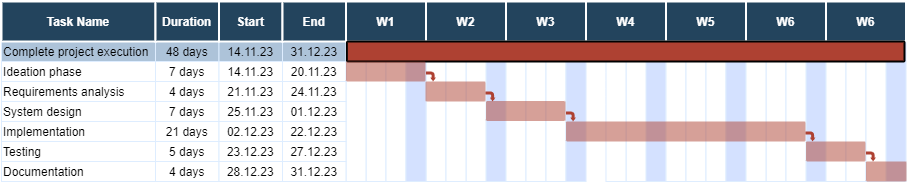
\includegraphics[width=1\textwidth, height=0.25\textwidth, scale=1]{img/Gantt.png}
    \caption{Gantt diagram}
    \label{Gantt}
\end{figure}

\section{System architecture and used technologies}
To achieve these objectives, it was chosen to use blockchain technology, which is a distributed register that provides data immutability and transparency, allowing every participant to access to the register and contribute with accurate data. The choice fell on Ethereum (figure \ref{Ethereum}) as the blockchain platform to implement this application for several reasons: firstly, it is one of the currently most established platforms with a highly active developer community, and also for its support of smart contracts. These are protocols that automatically execute pre-established agreements when certain conditions are met. In the agri-food supply chain, this means that contracts can automatically perform various activities without the need for intermediaries. Lastly, Ethereum ensures high scalability, making it a more sustainable choice for a distributed application requiring the recording and access to a large volume of real-time data.

\begin{figure}[ht]
    \centering
    \captionsetup[]{width=\textwidth}
    
\includegraphics[width=0.3\textwidth, height=0.3\textwidth, scale=1]{img/Ethereum-icon.png}
    \caption{Ethereum}
    \label{Ethereum}
\end{figure}

During the development activity on Ethereum, the Integrated Development Environment (IDE) called Remix (figure \ref{Remix}) was used, which is a rich toolset that can be used for the entire journey of contract development by users of any knowledge level, and as a learning lab for teaching and experimenting with Ethereum.

\begin{figure}[ht]
    \centering
    \captionsetup[]{width=\textwidth}
    
\includegraphics[width=0.3\textwidth, height=0.3\textwidth, scale=1]{img/Remix.png}
    \caption{Remix}
    \label{Remix}
\end{figure}

\section{Requirements}
In the ideation phase, the fundamental requirements that the distributed application had to meet were defined, thus creating a clear guide for subsequent development.

\subsection{Functional requirements}
\begin{itemize}
    \item The system must be able to enter a batch specifying its processing (environmental parameters, quality, etc.)
    %\item The system must be able to allow producers to enter production expenses by specifying their carbon credits
    \item The system must allow the input of the quantity and the storage time of the batches
    \item The system must be able to insert transactions made by various users (producers, consumers, etc.), specifying the type of transaction and price.
    \item The system must be able to provide the certification generated by specialized entities (laboratories) to those who want to purchase the batch.
    %\item The system must be accessible through various devices to verify product information at any given moment.
\end{itemize}

\subsection{Non functional requirements}

\subsubsection{Compatibility}
The platform will be accessible through various devices such as smartphones and tablets, allowing different users (buyers, consumers, producers, etc.) to verify at any time the origin, the product information, the chemical-physical characteristics of the product, the varietal origin, and monitor the product's agri-food supply chain through access to detailed information on the production phases, from sowing to sale, also including the transformation phases.

\subsubsection{Usability}
The system has the ambitious goal of maximizing usability and accessibility for users, aiming to provide a fluid and intuitive experience. For this purpose, user interfaces characterized by maximum simplicity and clarity will be adopted, in order to facilitate interaction and ensure easy use even for less experienced users.

\subsubsection{Security}
The server side implements a user registration system on the blockchain that allows verifying a user's presence and role based on their authorized actions.

Additionally, contracts are decoupled according to their functionalities, ensuring a greater separation of responsibilities.

%\subsubsection{Sustainability}
%The system must record and make available information on the overall usage of carbon credits by users. The objective is to encourage significant offsetting of carbon emissions generated by blockchain transactions across the entire platform, promoting eco-friendly practices and environmental responsibility.

\section{UML diagram}
This section examines the UML diagram (figure \ref{UML}, \ref{UMLblockchain}) that represents the structure of the classes in the system. Using the UML diagram is critical to clearly display relationships between classes, identify responsibilities, and facilitate understanding of the overall structure of the system. The diagram, which follows the UML class paradigm, covers crucial aspects of the system and will provide a visual guide for the development and maintenance of the project.

\begin{figure}[ht]
    \centering
    \captionsetup[]{width=\textwidth}
    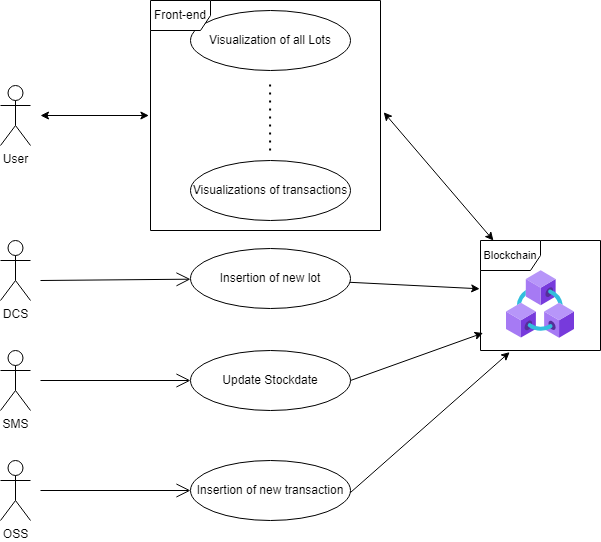
\includegraphics[width=1\textwidth, height=.8\textwidth, scale=1]{img/UML.png}
    \caption{UML diagram}
    \label{UML}
\end{figure}

\begin{figure}[ht]
    \centering
    \captionsetup[]{width=\textwidth}
    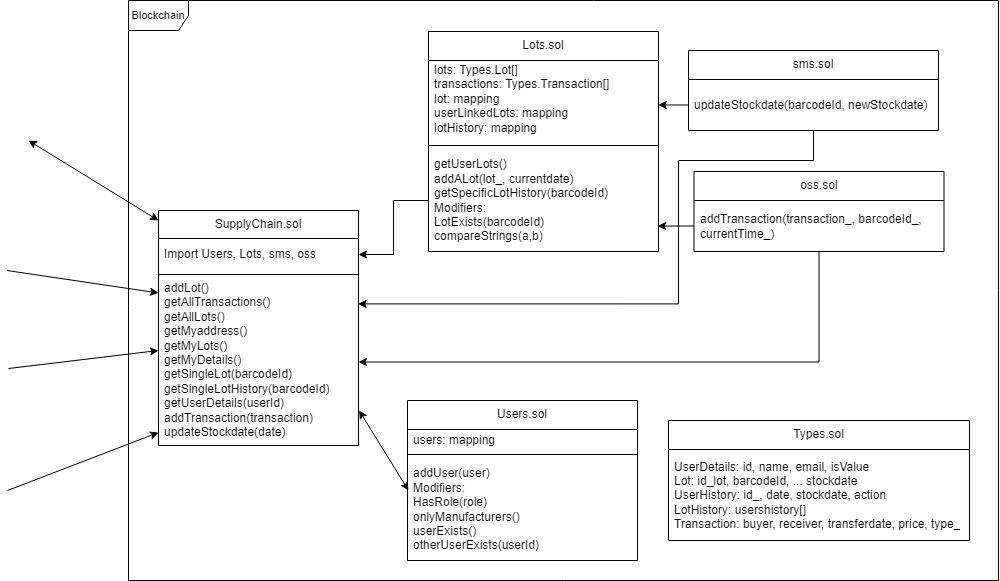
\includegraphics[width=1\textwidth, height=.5\textwidth, scale=1]{img/UMLblockchain.png}
    \caption{UML blockchain diagram}
    \label{UMLblockchain}
\end{figure}
